% ###################################
%      NON LINEAR CHROMATICITY
\section{Non-Linear Chromaticity}



% ===============================
%         Introduction
% ===============================
\subsection{Introduction}

% Expression
\paragraph{Expression}

Chromaticity is the tune shift $\Delta Q_{x,y}$ dependent on the momentum offset $\delta$ of a
particle. Its general expression is given by a Taylor expansion
in~\cref{eq:background_chromaticity}. The full third term is highlighted in the following,

\begin{equation} 
    Q (\delta) = Q_0 + Q' \delta + \frac{1}{2!} Q'' \delta^2 
                     + \colorbox{yellow!50}{$\displaystyle  \frac{1}{3!}  Q''' \delta^3$}
                     + \mathcal{O}(\delta^4).
\end{equation}

This third order is mainly contributed to by decapoles. It is related to the $\beta$-function, the
dispersion and the strength of the multipole, also shown
in~\cref{eq:detuning_effects:chromaticity_strength}:

\begin{equation}
    \begin{aligned}
        \Delta Q_x''' &=  &\frac{1}{4\pi} K_{5} L \beta_x D_x^{3}\\
        \Delta Q_y''' &= -&\frac{1}{4\pi} K_{5} L \beta_x D_x^{3}.
    \end{aligned}
\end{equation}


% Correction
\paragraph{Correction}

$Q'''$ is linear with the decapole strength. As such, it can be easily corrected via global trims
presented in~\cref{subsection:correction_chromaticity}.
A change of decapole strength $K_5 = 1000$ would for example have the following impact with the
injection optics used in 2022:

\begin{equation}
    \begin{aligned}
        \Delta Q'''_x =  1.5 \times 10^6 \quad;\quad
        \Delta Q'''_y = -0.9 \times 10^6.
    \end{aligned}
\end{equation}




% ===============================
%         Measurement
% ===============================
\subsection{Measurement}
\label{subsection:decapoles:chromaticity:measurement}

Chromaticity is measured by varying the frequency of the radio-frequency (RF) cavities, used to
create buckets and to accelerate the beam. The change in $\delta$ related to this frequency is, as a
reminder:

\begin{equation}
    \delta = - \frac{1}{\alpha_c} \cdot \frac{\Delta f_{RF}}{f_{RF,nominal}}.
\end{equation}

More details on the measurements and analysis principles can be found in
earlier~\cref{subsection:optics_corrections_chromaticity}.



% ========== Momentum Compaction Factor
\subsubsection{\review{Momentum Compaction Factor}}

Rather than a constant, the momentum compaction factor can be expressed as an
expansion, as detailed in~\cref{subsection:coordinates_systems:momentum_compaction_factor}.
The first terms are given by the following,

\begin{equation}
    \alpha_c = 
    \underbrace{\alpha_{c,0}}_{1^\text{st} \text{ order}}
    + \underbrace{\alpha_{c,1} \delta}_{2^\text{nd} \text{ order}}
    + \underbrace{\alpha_{c,2} \delta^2}_{3^\text{rd} \text{ order}}.
\end{equation}

The expression for $\delta$ at first and second order then reads,

\begin{equation}
    \begin{aligned}
        \delta &= -\frac{\Delta f_{RF}}{\alpha_{0} f_{RF}} && \Rightarrow \text{Order 1} \\
        \delta &= \frac{- \alpha_{0} f_{RF} + \sqrt{f_{RF} 
            \left(- 4 \Delta f_{RF} \alpha_{1} + \alpha_{0}^{2} f_{RF}\right)}}{2 \alpha_{1} f_{RF}}
            && \Rightarrow \text{Order 2} 
    \end{aligned}
\end{equation}

It is assumed that only the first term is relevant as the induced difference in chromaticity is
negligible as will be demonstrated later on.
\cref{fig:decapoles:chromaticity:momentum_compaction_factor} shows the non linearity of the momentum
compaction factor and its effect on the calculated $\delta$ via the previous formulas.

\begin{figure}[tbh]
    \centering
    \begin{subfigure}[t]{0.48\textwidth}
        \centering
        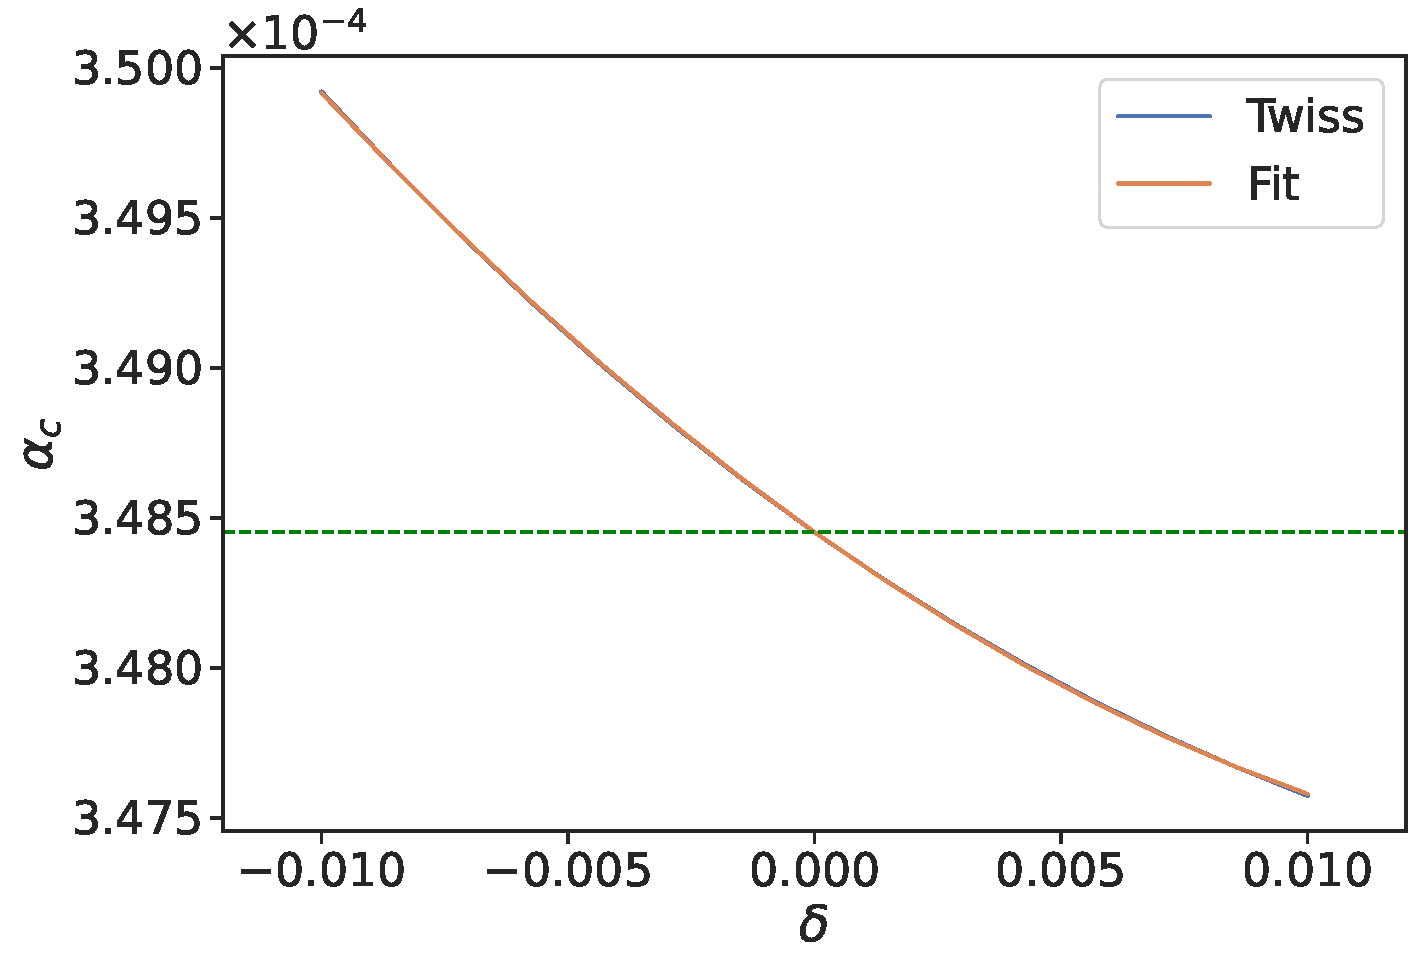
\includegraphics[width=\textwidth]{images/higher_order_momentum_compaction_factor.pdf}
        \caption{Non-linear fit of $\alpha_c$ obtained via an evaluation at discrete $\delta$ in
        MAD-X. The green line represents a constant $\alpha_c = \alpha_{c,0}$.}
    \end{subfigure}
    \hfill
    \begin{subfigure}[t]{0.48\textwidth}
        \centering
        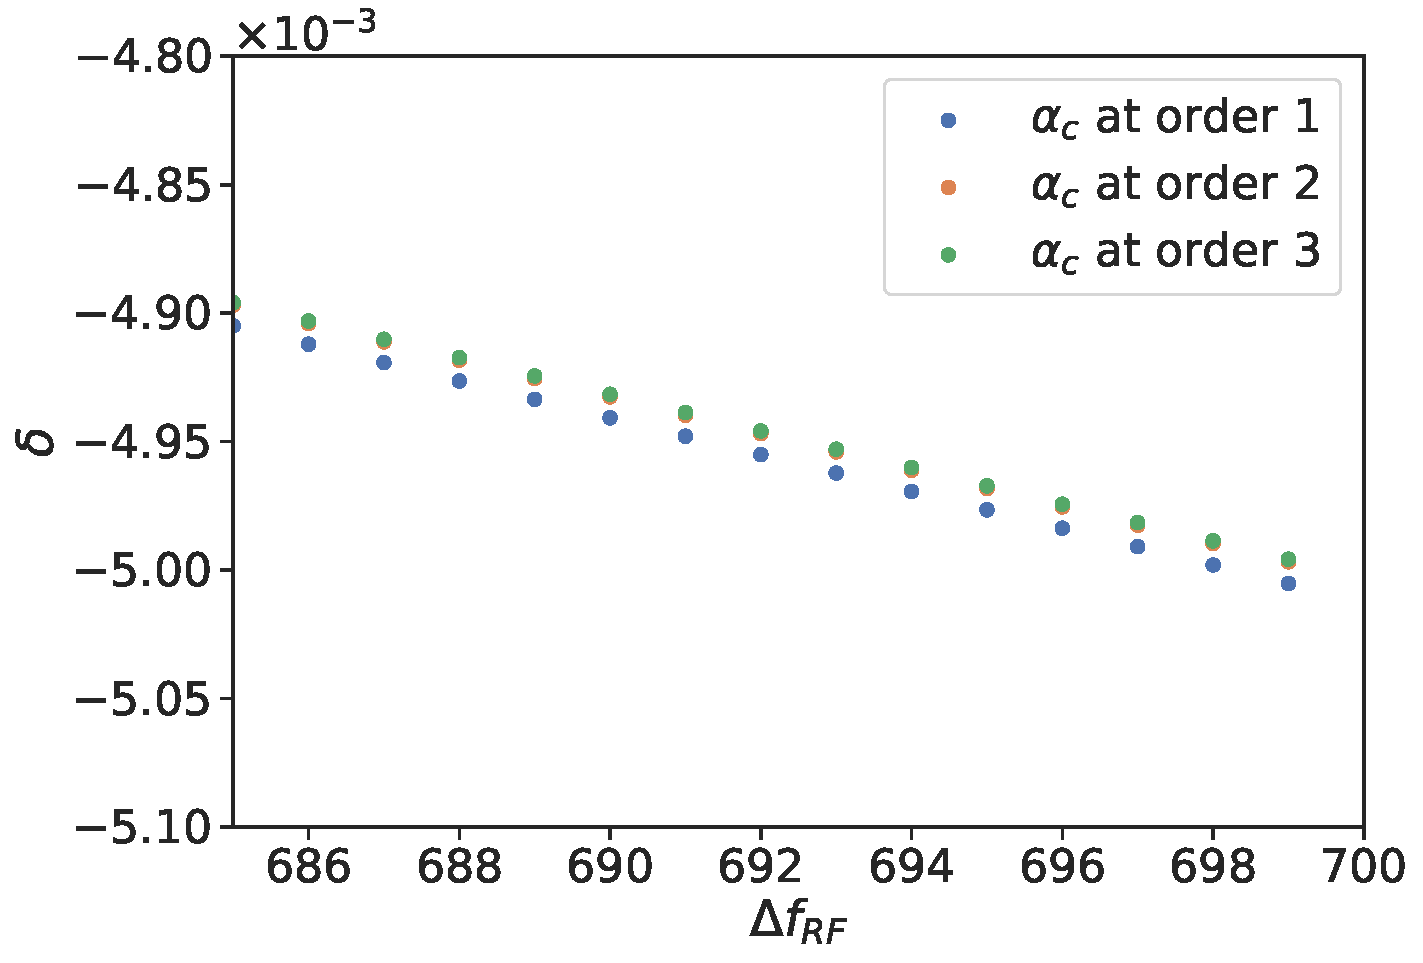
\includegraphics[width=\textwidth]{images/delta_vs_frf_alpha_c.pdf}
        \caption{Divergence of the momentum offset when considering higher $\alpha_c$ orders with
        large RF trims.}
    \end{subfigure}
    \caption{Non linearity of $\alpha_c$ and its effect on the computed $\delta$ via RF trims. The
    simulations are done at injection energy of 450GeV.}
    \label{fig:decapoles:chromaticity:momentum_compaction_factor}
\end{figure}

It is observed that while clearly depending on higher orders, the momentum compaction factor only
has a small impact on the calculated $\delta$.
\cref{fig:decapoles:chromaticity:momentum_compaction_factor_chroma_meas} shows a real-life 
measurement, comparing the fit of the chromaticity function with various $\delta$, computed up to
the third order of $\alpha_c$.

\begin{figure}[tbh]
    \centering
    \begin{subfigure}[t]{0.48\textwidth}
        \centering
        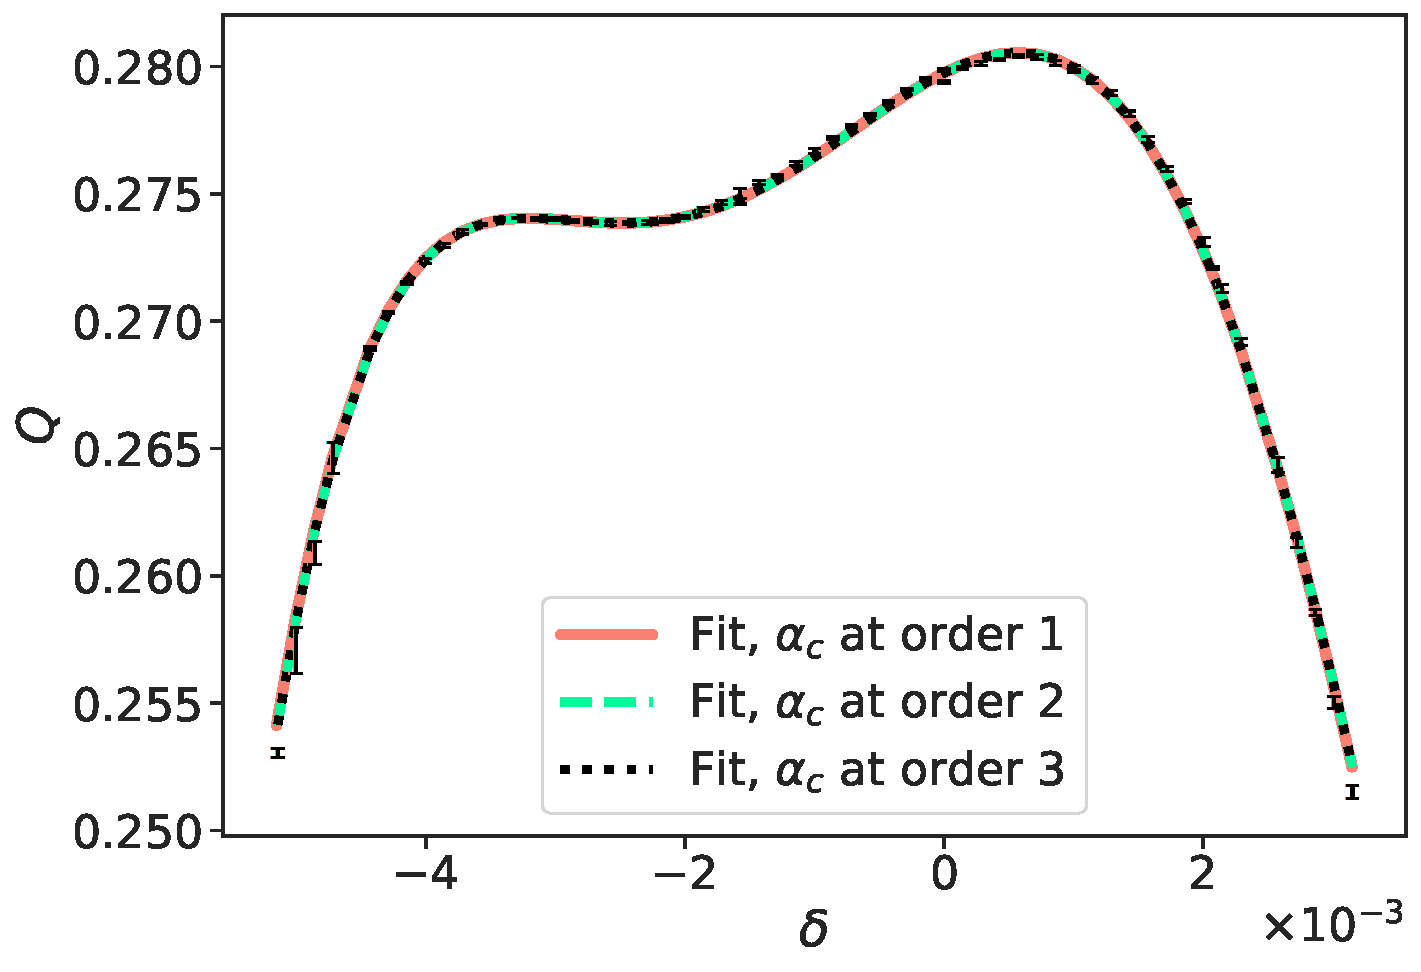
\includegraphics[width=\textwidth]{images/chroma_function_alpha_c.pdf}
        \caption{Fit of the chromaticity function at the $5^{\text{th}}$ order, considering the
        $\alpha_c$ expansion up to the third order.}
    \end{subfigure}
    \hfill
    \begin{subfigure}[t]{0.48\textwidth}
        \centering
        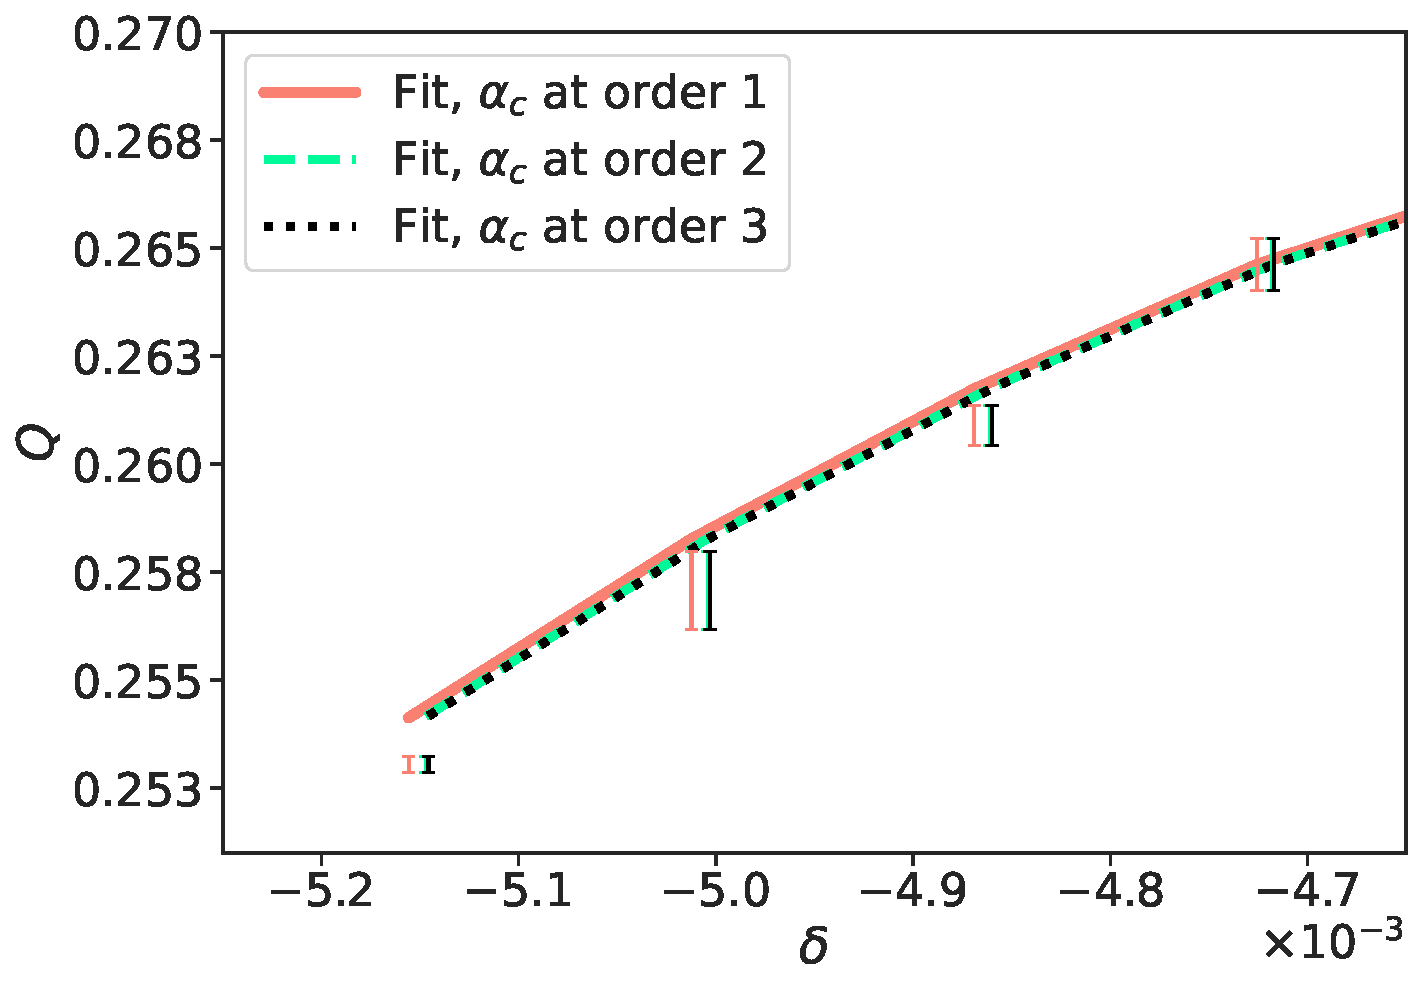
\includegraphics[width=\textwidth]{images/chroma_function_alpha_c_zoom.pdf}
        \caption{Zoom on one side of the fit. The difference between the second and third order
        is barely noticeable.}
    \end{subfigure}
    \caption{Fit of the chromaticity function considering several $\alpha_c$ orders.}
    \label{fig:decapoles:chromaticity:momentum_compaction_factor_chroma_meas}
\end{figure}

The fit of the chromaticity function is barely impacted when considering the higher orders of the 
momentum compaction factor. The different orders of the chromaticity are collected
in~\cref{table:decapoles:chromaticity:alpha_c_chroma}.
The higher order terms of $\alpha_c$ can thus be neglected and are not a source of higher
chromaticity orders.

\begin{table}[tbh]
    \begin{tabular}{c|ccccc}
        $\alpha_c$ Order & $Q^{(1)}$ & $Q^{(2)}$ & $Q^{(3)}$ & $Q^{(4)}$ & $Q^{(5)}$\\
        \hline
        1 & 2.52 ± 0.03 & -3.04 ± 0.05 & -4.75 ± 0.03 & -0.33 ± 0.07 & 2.33 ± 0.06 \\
        2 & 2.53 ± 0.03 & -3.05 ± 0.05 & -4.75 ± 0.03 & -0.32 ± 0.07 & 2.36 ± 0.06 \\
        3 & 2.53 ± 0.03 & -3.05 ± 0.05 & -4.75 ± 0.03 & -0.32 ± 0.07 & 2.36 ± 0.06 \\
        \end{tabular}
    \caption{}
    \label{table:decapoles:chromaticity:alpha_c_chroma}
\end{table}



% ========== Noisy Tune
\subsubsection{Noise and Spectral Lines}

Noise lines, due to electronics, can be seen in the raw data obtained from the BBQ tune system.
Occasionally, when those resonances are strong, their frequency peak can be mistaken as the tune and
logged as such by the system. This yield large uncertainties in the measurement when data points 
can't properly be classified as outliers. A tune measurement presenting this issue is showed in 
\cref{fig:decapoles:chromaticity:noisy_tune}.

\begin{figure}[tbh]
    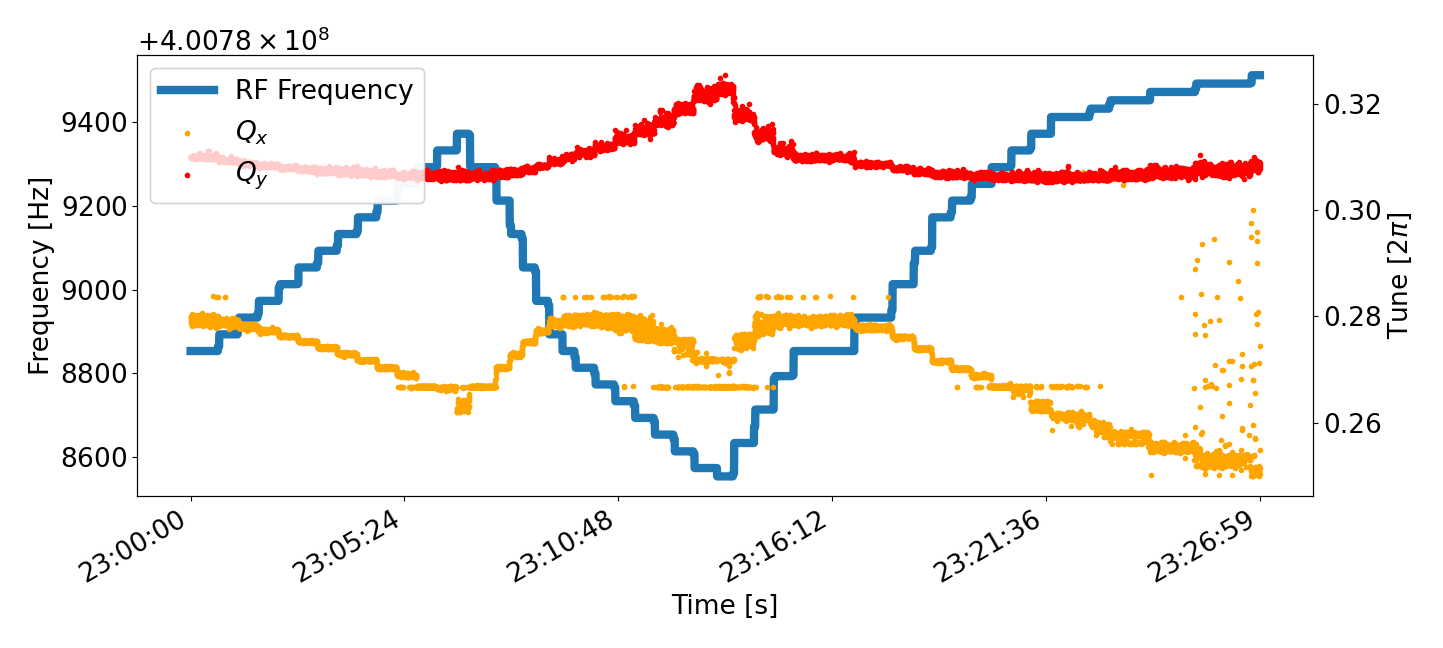
\includegraphics[width=\textwidth]{./images/noisy_tune.png}
    \caption{Shift of the tune by variation of the RF. Noise lines can appear in some cases,
    making the tune error bar large or downright unusable.}
    \label{fig:decapoles:chromaticity:noisy_tune}
\end{figure}

A solution to this issue is to use the raw data extracted from the BBQ system. From there, a
spectrogram clearly shows the noise lines, as seen in \cref{fig:decapoles:chromaticity:spectrogram}.
Those lines have been repeatedly identified over several measurements and confirmed to be fixed.
The highest peak of the spectrogram can thus be safely identified by removing those resonances,
yielding a cleaner measurement. It is also to be added that the BBQ requires to set a tune window,
which can be forgotten. By analyzing the raw data, it is ensured that the measurement has usable
data and does not try to measure noise.

\begin{figure}[tbh]
    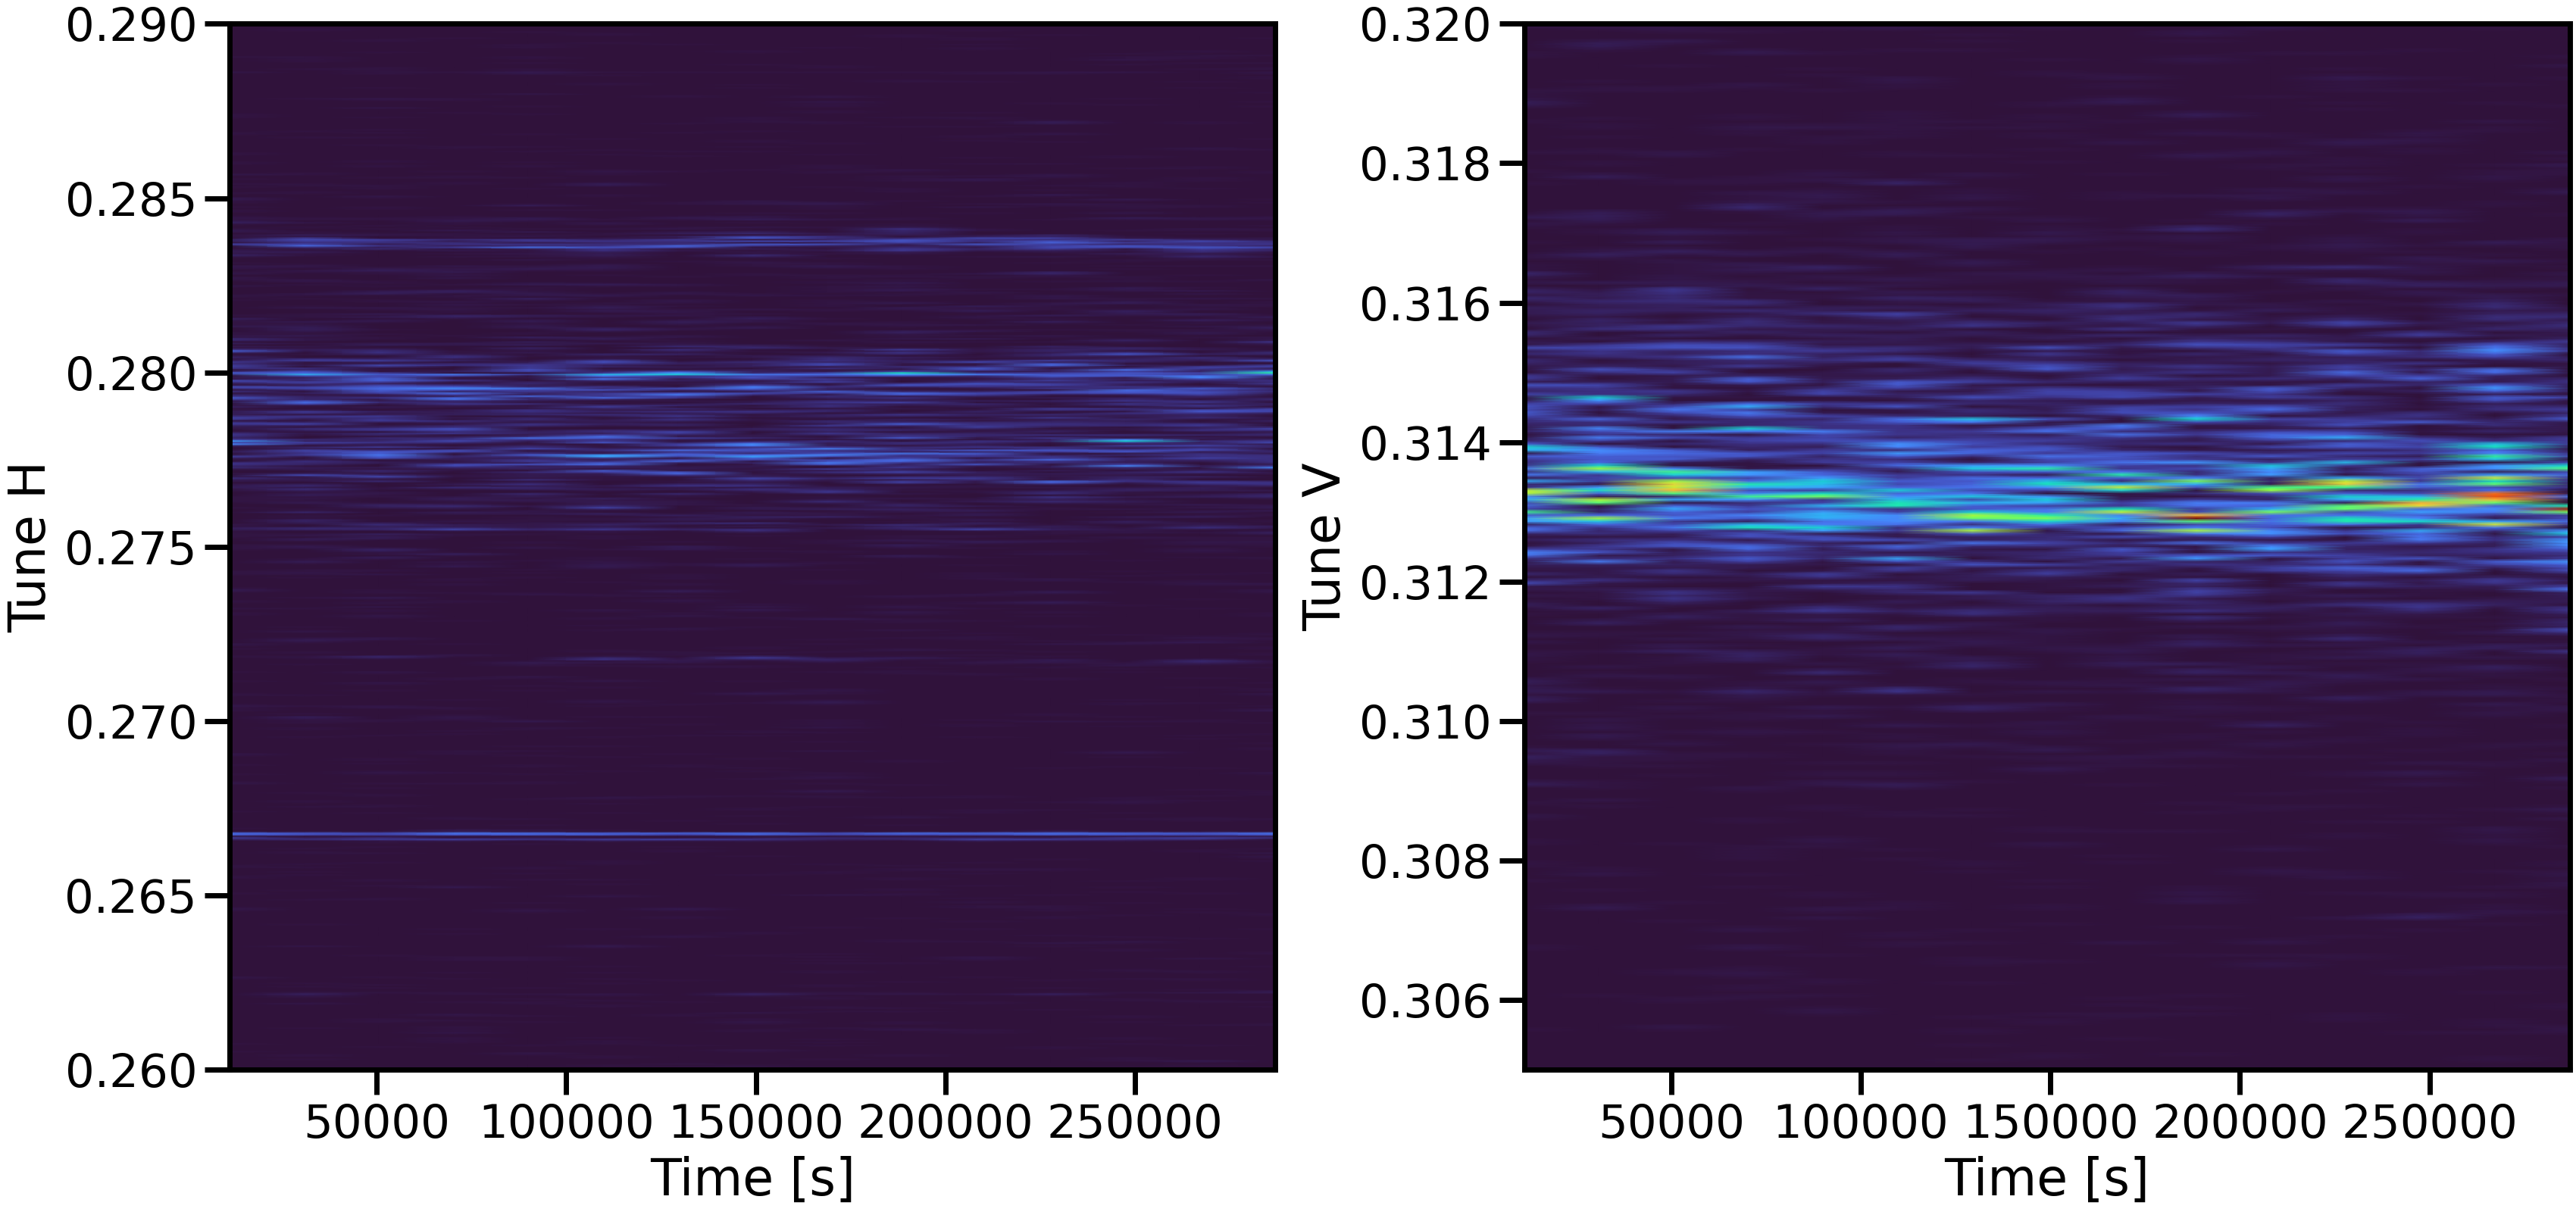
\includegraphics[width=\textwidth]{./images/spectrogram.png}
    \caption{Tune spectrogram obtained via BBQ system. Strong resonance lines can be seen above and
    below where the tune really is, causing the wrong frequency peak to be identified as the tune.}
    \label{fig:decapoles:chromaticity:spectrogram}
\end{figure}


% ========== Other way of measuring delta
\subsubsection{\todo{Other $\delta$ measurements}}

The previous equation is not the only way to measure the momentum offset.
\\\todo{
    give details\\
    radial loop\\
    schottky?
}


%\subsection{\todo{blabla}}
%
%Measurements were taken during 2022 Commissioning for 
%\begin{itemize}
%    \item Beam Test
%    \item Commissioning
%    \begin{itemize}
%        \item FiDeL
%        \item Q''' corr
%        \item Q'' corr
%    \end{itemize}
%    \item 60° optics
%\end{itemize}
%
%Also during MD6864, 2022-10-19, for the bare machine \\
%Also 2022-11-06, measurement at 30cm, flat top.
%

% ===============================
%        Corrector Response
% ===============================
\subsection{\review{Response of correctors}}

% 2022-04-24

In order to assess the accuracy of corrections, measurements have to be done to gauge the response
of the decapolar correctors, \textit{MCDs}.
Such measurements are routinely done as a by-product of the corrections done during commissioning.
\cref{figure:decapoles:chromaticity:dq3_comparison} shows the chromaticity function measured during
Run~3's commissioning in 2022 with the nominal corrections via FiDeL and beam-based corrections
computed analytically based on top of FiDeL.

\begin{figure}[tbh]
    \centering
    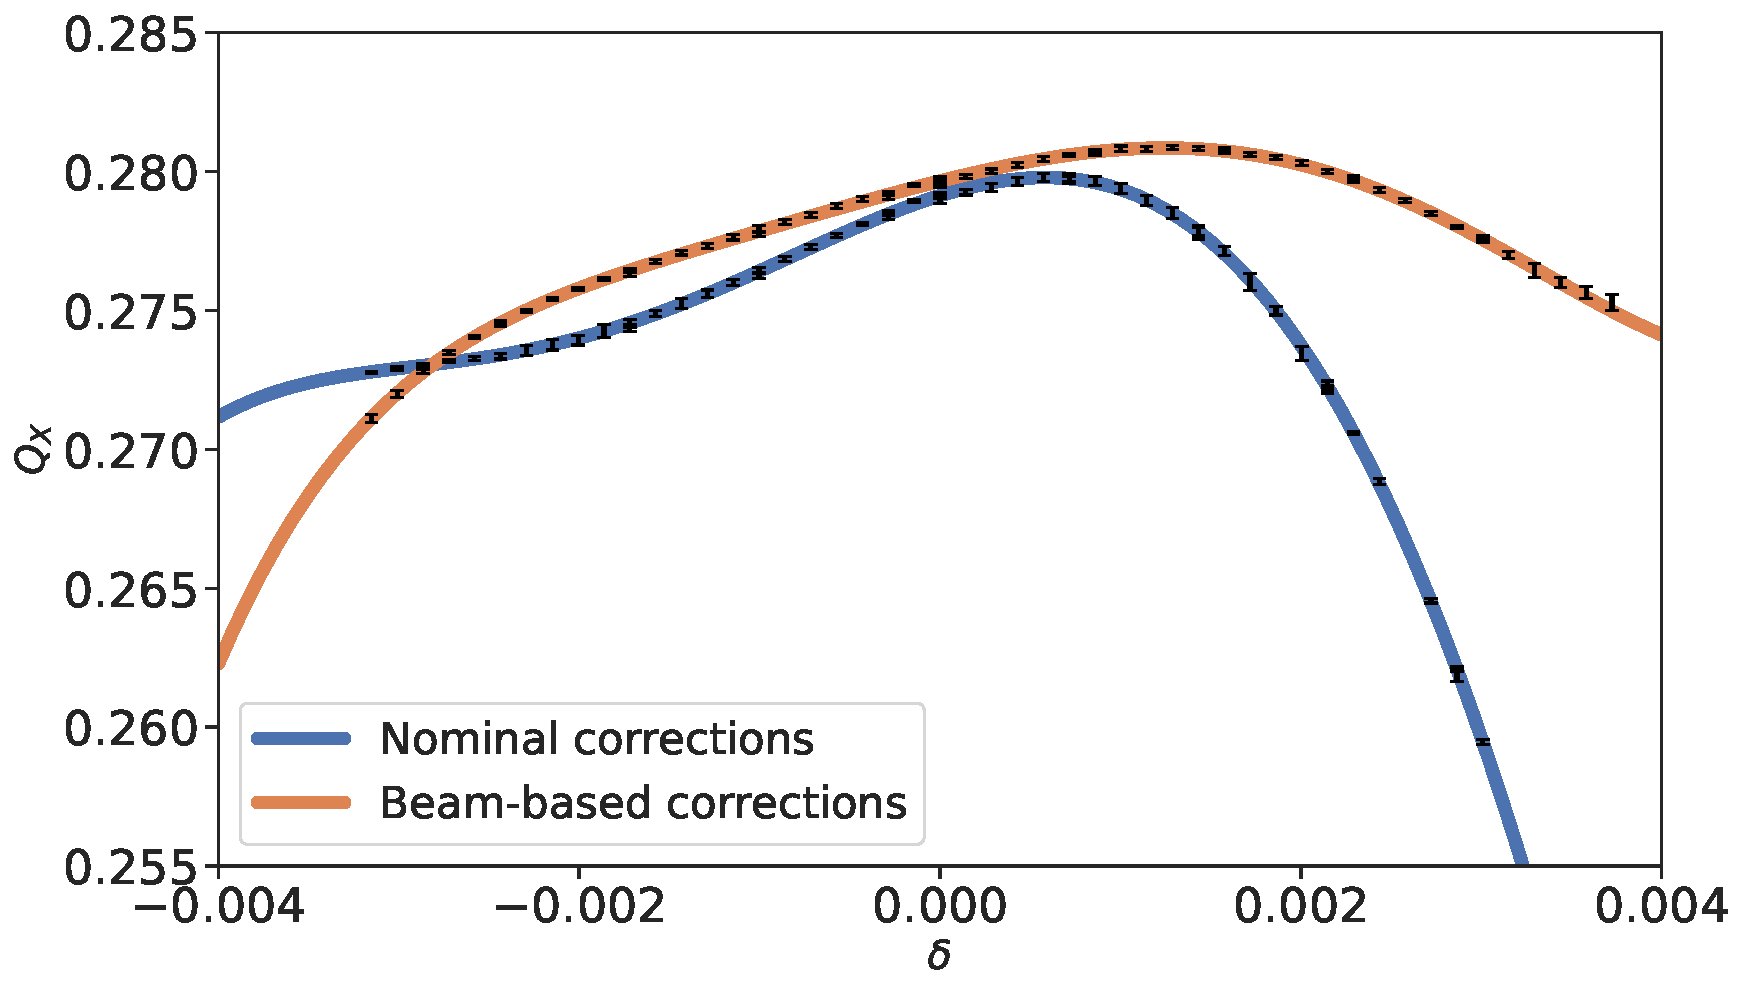
\includegraphics[width=0.8\columnwidth]{images/nominal_vs_beam_based_corrections.pdf}
    \caption{Chromaticity of the horizontal plane of Beam 1 during Run 3's commissioning, with
    nominal corrections based on the magnetic model and beam-based corrections aimed at correcting
     $Q''$ and $Q'''$.}
    \label{figure:decapoles:chromaticity:dq3_comparison}
\end{figure}

The nominal and corrected $Q'''$ values are shown in
\cref{table:decapoles:chromaticity:dq3_before_after_beam_based}. The shift in $Q'''$ is shown for
each beam and axis, showing a good agreement between the measurement and the simulation.
The slight imbalance can be attributed to higher order effects of the octupole correctors, whose
correction was implemented after that of $Q'''$.

\begin{table}[tbh]
    \centering
    \begin{tabular}{|l||r|r|r|c|}
    \hline
              &  \multicolumn{2}{c|}{$Q''' [10^6]$}  &  \multicolumn{2}{c|}{$\Delta Q''' [10^6]$}\\ \hline\hline
        B1    &   \multicolumn{1}{c|}{Nominal}     &   \multicolumn{1}{c|}{Beam-based}   & Measured & Simulated \\
        X     &  -3.36 ± 0.04 &  -1.02 ± 0.03  &  2.3 ± 0.1 &   2.5 \\
        Y     &   1.62 ± 0.05 &   0.12 ± 0.02  & -1.5 ± 0.1 &  -1.4 \\ \hline
        %B2    &   \multicolumn{1}{c|}{Nominal}     &   \multicolumn{1}{c|}{Beam-based}   &&\\
        B2    &               &&& \\
        X     &  -2.72 ± 0.08 &  -0.64 ± 0.03  &  2.1 ± 0.1 &  2.5\\
        Y     &   1.54 ± 0.06 &   0.14 ± 0.03  & -1.4 ± 0.1 & -1.4\\ \hline
    \end{tabular}
    \caption{Third order chromaticity obtained during Run~3 commissioning, with nominal and
    beam-based corrections aimed at correcting $Q''$ and $Q'''$.
    The change in $Q'''$, measured and expected via simulations, is also shown.} 
    \label{table:decapoles:chromaticity:dq3_before_after_beam_based}
\end{table}


This agreement between the simulations and the measurements indicates that our decapole correctors
function as intended. No noticeable cross-talk between magnets or hysteresis have been identified.


% ===============================
%        Bare Chromaticity
% ===============================
\subsection{\review{Bare Chromaticity}}

% 2022-10-19

Previous studies~\cite{maclean_measurement_2014} have demonstrated that octupole and decapole
correctors were contributing to an observed octupolar discrepancy in the machine via hysteresis and
feed-down. To evaluate the possible effect of decapole correctors on the third order chromaticity
$Q'''$, a measurement was taken with these elements turned off.

\begin{figure}[tbh]
    \begin{subfigure}{0.49\textwidth}
        \centering
        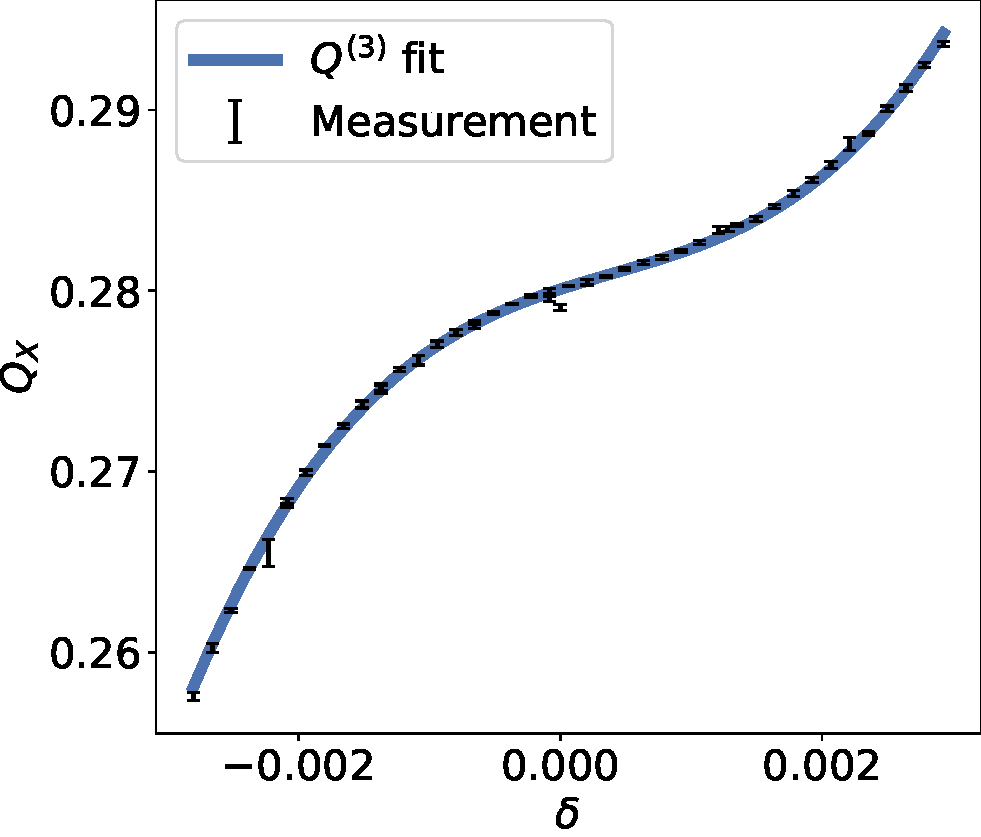
\includegraphics[width=\textwidth]{./images/bare_chromaticity/Beam1_Qx.pdf}
        \caption{$Q_x$ Beam 1}
        \label{}
    \end{subfigure}
    \hfill
    \begin{subfigure}{0.49\textwidth}
        \centering
        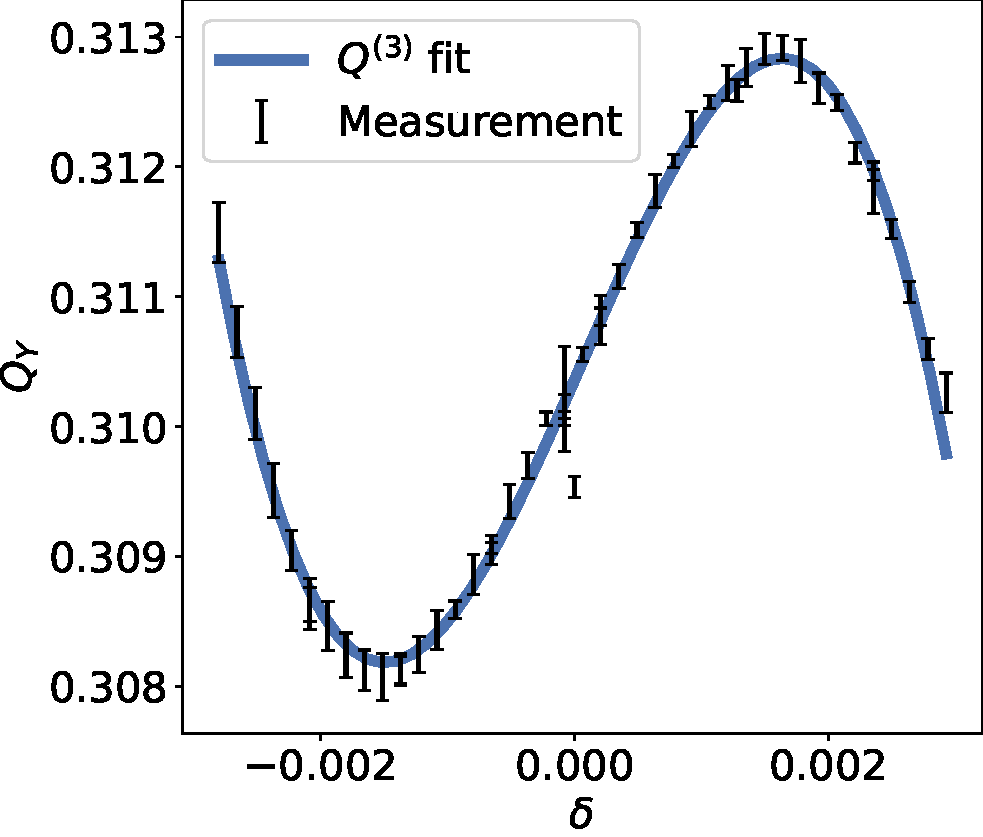
\includegraphics[width=\textwidth]{./images/bare_chromaticity/Beam1_Qy.pdf}
        \caption{$Q_y$ Beam 1}
        \label{}
    \end{subfigure}
    %
    \\
    %
    \begin{subfigure}{0.49\textwidth}
        \centering
        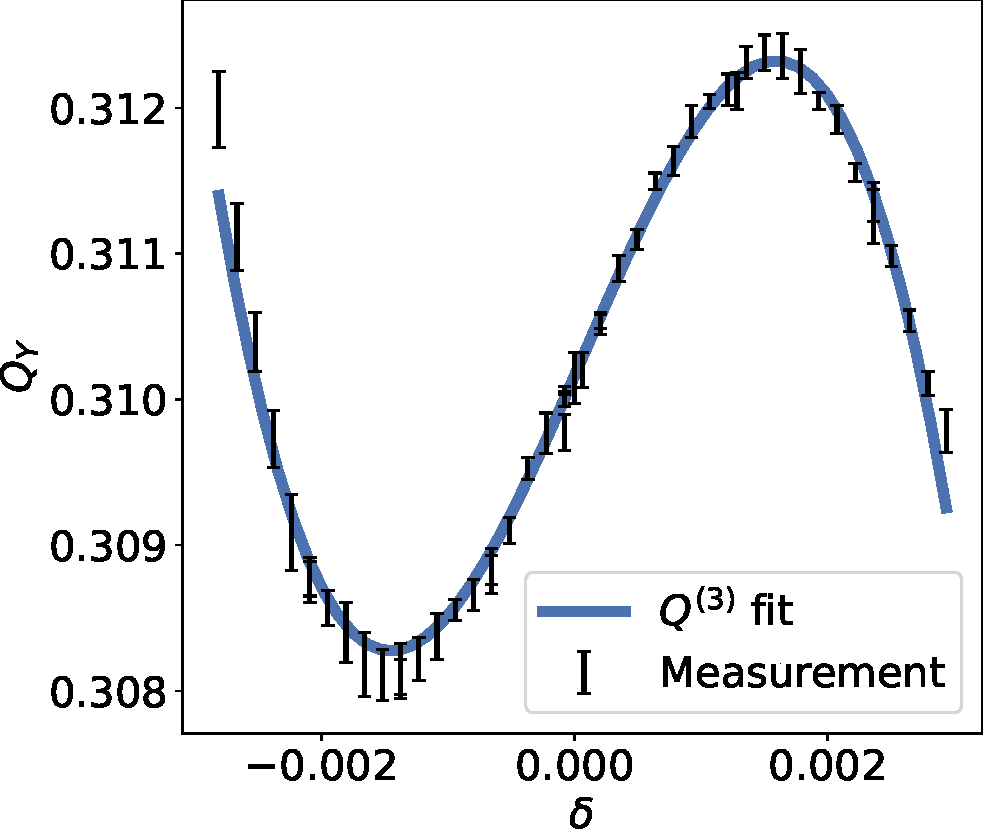
\includegraphics[width=\textwidth]{./images/bare_chromaticity/Beam2_Qy.pdf}
        \caption{$Q_x$ Beam 2}
        \label{}
    \end{subfigure}
    \hfill
    \begin{subfigure}{0.49\textwidth}
        \centering
        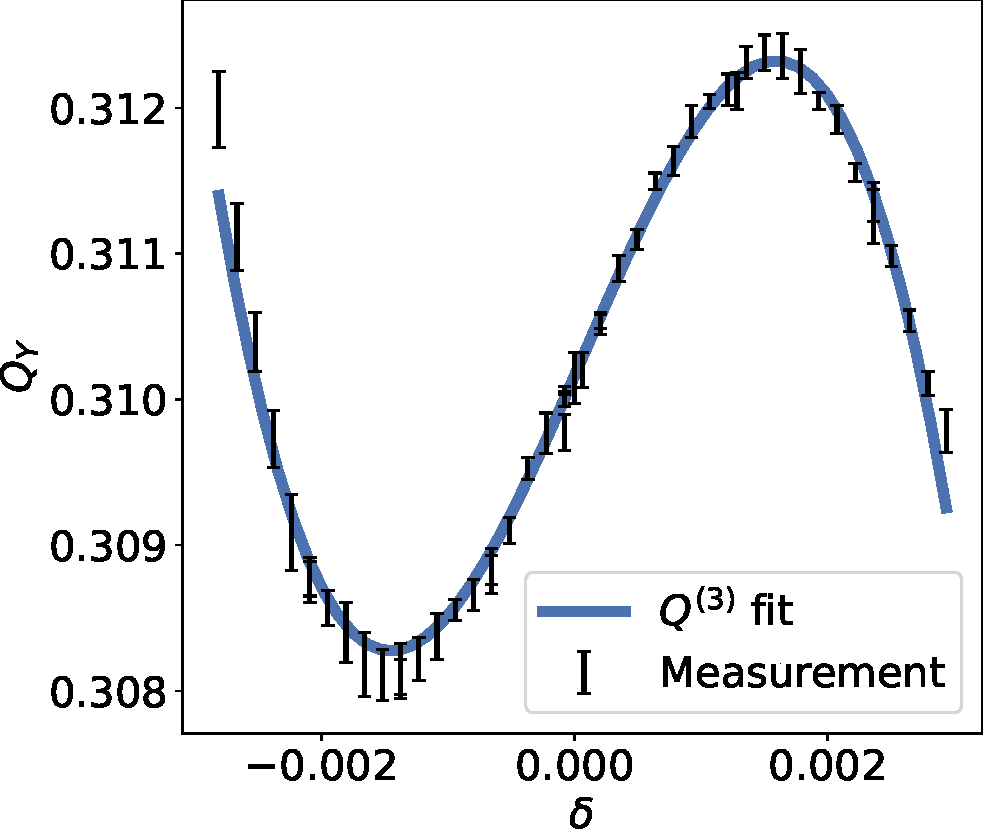
\includegraphics[width=\textwidth]{./images/bare_chromaticity/Beam2_Qy.pdf}
        \caption{$Q_y$ Beam 2}
        \label{}
    \end{subfigure}
    \caption{Fit of the chromaticity function for the chromaticity measurement performed with 
    octupole and decapole correctors powered off. The fit includes all orders up to third.}
    \label{fig:decapoles:bare_chromaticity}
\end{figure}

Simulations have been run with MAD-X and PTC including fields errors from $b_3$ to $b_8$. The
expected $Q'''$ values are presented in~\cref{table:decapoles:bare_chromaticity:virgin_dq3} and
compared to the measured ones along with the ratio between the two.

\begin{table}[tbh]
    \centering
    \begin{tabular}{|l||r|r|r|}
    \hline
        Plane     &  Meas. $Q''' [10^6]$        &  Sim. $Q''' [10^{6}]$          &   Ratio     \\\hline\hline
        Beam 1    &                             &                                &             \\
                X &            2.95 ± 0.04      &         6.94 ± 0.02            &  0.43 ± 0.01  \\
                Y &           -1.82 ± 0.04      &        -4.29 ± 0.01            &  0.42 ± 0.01  \\ \hline
        Beam 2    &                             &                                &             \\
                X &            3.06 ± 0.07      &        7.03 ± 0.02             &  0.44 ± 0.01 \\
                Y &           -1.72 ± 0.02      &       -4.27 ± 0.01             &  0.42 ± 0.01  \\ \hline
    \end{tabular}
    \caption{Measured and simulated third order chromaticity with octupole and decapole correctors
    turned off. The simulations include field errors from sextupoles to decahexapole ($b_3$ to
    $b_8$).}
    \label{table:decapoles:bare_chromaticity:virgin_dq3}
\end{table}

A consistent ratio is observed for every plane and axis between the measurement and the model. This
result, supplemented by the correct response of the correctors, indicates that the decapolar
correctors do no generate unwanted fields. Those correctors can thus be discarded as the potential
source of discrepancy.